\documentclass{llncs}
\usepackage{color}
\usepackage{soul}
\usepackage{cite}
\usepackage{array}
\usepackage{listings}
\usepackage{graphicx}
\usepackage{amsfonts}
\usepackage{amsmath, amsfonts, url, amssymb, graphics, algorithm2e} 

\usepackage{url}
\newcommand{\starpar}[1]{\par{\footnotesize $\star$ \hl{#1}\par}}
\newcommand{\F}{{\mathbb F}}
\newcommand{\Z}{{\mathbb Z}}

\lstset{basicstyle=\scriptsize,breaklines=true,breakindent=60pt,xleftmargin=20pt,numberstyle=\tiny,numbersep=5pt,language=C}

\begin{document}

\title{Recovering OpenSSL ECDSA Nonces Using the \textsc{Flush+Reload} Cache Side-channel Attack}
\author{Yuval Yarom \and Naomi Benger}
\institute{The University of Adelaide}

\maketitle

\begin{abstract}
<<<<<<< HEAD
In this paper we illustrate a vulnerability introduced to elliptic curve cryptographic protocols when implemented using a function of the OpenSSL cryptographic library. For a given implementaion using an elliptic curve $E$ over a binary field with a point $G\in E$, our attack can recover the majority of the bits of a scaler $k$ when $kG$ is computed using the OpenSSL implementation of the Montgomery ladder. For the Elliptic Curve Digital Signature Algorithm (ECDSA) the scalar $k$ is intended to remain secret. Our attack recovers the scalar $k$ and thus the secret key of the signer and would therefor allow unlimited forgeries. This is possible from snooping on only one signing process and requires computation of less than one second on a quad core desktop when the scalar $k$ (and secret key) is around 571 bits.
=======
In this paper we illustrate a vulnerability introduced to elliptic curve cryptographic protocols when implemented using a function of the OpenSSL cryptographic library. For a given implementation using an elliptic curve $E$ over a binary field with a point $G\in E$, our attack can recover the majority of the bits of a scaler $k$ when $kG$ is computed using the OpenSSL implementation of the Montgomery ladder. For the Elliptic Curve Digital Signature Algorithm (ECDSA) the scalar $k$ is intended to remain secret. Our attack recovers the scalar $k$ and thus the secret key of the signer and would therefor allow unlimited forgeries. This is possible from snooping on only one signing process and requires computation of less than one second on a quad core desktop when the scalar $k$ is around 571 bits.
>>>>>>> 5aff1691280461ac6cd6e8d08fd2c2f6029fbf22

\end{abstract}

\section{Introduction}
Elliptic curve cryptography (ECC)~\cite{miller85use,koblitz87elliptic} includes a number of public-key cryptographic protocols whose security relies on the computational intractability of the Elliptic Curve Discrete Logarithm Problem (ECDLP).
In a nutshell, given an elliptic curve over a finite field and two points on the curve~$G$ and~$H$, the ECDLP is to find the scalar $k$ such that $H=kG$.

ECC offers a higher encryption strength per key-bit than related methods with security reliant on the hardness of computing discrete logarithms in finite field or factoring the product of large primes.
Consequently, ECC uses significantly shorter keys and offers faster operations than other methods, contributing to its rising popularity.

The Elliptic Curve Digital Signature Algorithm (ECDSA)~\cite{johnson01elliptic,fips186,ansi962} is a standard
<<<<<<< HEAD
digital signature algorithm implemented using elliptic curves. One core operation of the ECDSA algorithm, as in many ECC protocols, is the scalar myltiplication of a point on the elliptic curve by a pseudo-randomly generated secret nonce. The confidentiality of the nonce is paramount for the security of the algorithm. Past research indicates that partial exposure of nonce bits can be exploited for efficient attacks on the secret key~\cite{nguyen03insecurity,brumley11remote}.
=======
digital signature algorithm based on elliptic curves. One core operation of the ECDSA algorithm, as in many ECC protocols, the scalar multiplication of a point on the elliptic curve by a pseudo-randomly generated secret nonce. The confidentiality of the nonce is paramount for the security of the algorithm. Past research indicates that partial exposure of nonce bits can be exploited for efficient attacks on the secret key~\cite{nguyen03insecurity,brumley11remote}.
>>>>>>> 5aff1691280461ac6cd6e8d08fd2c2f6029fbf22

OpenSSL~\cite{openssl} is a cryptographic software package that implements ECDSA.
When using elliptic curves over a binary field $\mathbb{F}_{2^m}$, OpenSSL uses the 
Montgomery ladder~\cite{montgomery87speeding,joye03montgomery} algorithm to compute $kG$, scalar multiplication of a publically known point $G$ by the nonce $k$.
One of the advantages of the Montgomery ladder is that it has regular behaviour, performing
the same sequence of operations for each nonce bit, irrespective of the value of the bit.
This regular behaviour makes it more resilient to side-channel attacks~\cite{joye03montgomery,okeya00elliptic}.

While the operations performed by the algorithm are regular, their targets depend on the value of the bits of the nonce.
To apply the operations to the respective targets, the OpenSSL implementation uses a conditional branch based on the value of the bit. By tracing this branch an attacker can recover the values of the nonce bits and, consequently, break the cryptosystem. In this paper we present our use of the \textsc{Flush+Reload} cache side-channel attack~\cite{yarom13flush} to trace the branch in the OpenSSL implementation.

The \textsc{Flush+Reload} attack exploits a security weakness in the IA-32 and X86-64 architectures that allows processes
to monitor other processes read and execute access to shared memory pages.
Our attack program monitors access to both arms of the conditional branch and uses the information
collected from these probes to reconstruct the nonce. This attack is a threat to the security of any cryptographic protocol implemented using the OpenSSL scalar multiplication method, when the attacker has access to the target computer's memory. In this paper we illustrate the efficiency of the atttack by analysing ECDSA and recovering the secret key using only one signature at very little computational cost (in both time and memory).

The paper also presents new information on the limitation of the \textsc{Flush+Reload} attack.
We discuss spatial limitations, affecting the distance between multiple probes, and 
temporal limitations, affecting the probe resolution.

The results of this paper also support the findings of~\cite{walter04longer} that longer keys render a cryptographic algorithm more vulnerable to side-channel analysis.


<<<<<<< HEAD
The rest of this paper is organised as follows. The next section presents background information on elliptic curves, ECDSA, the Montgomery ladder and the \textsc{Flush+Reload} attack followed by a short discussion of related research.% and the validity of the assumption that an attacker has access to the computer's memory.
=======
The rest of this paper is organised as follows. 
The next section presents background information on elliptic curves, ECDSA, 
the Montgomery ladder and the \textsc{Flush+Reload} attack followed by a short discussion of related research.
>>>>>>> 5aff1691280461ac6cd6e8d08fd2c2f6029fbf22
Section~\ref{sec:attack} describes our attack on the OpenSSL implementation of ECDSA.
The results of the attack are analysed in Section~\ref{sec:results}.
We discuss the implications of the attack and suggest techniques for mitigation in Section~\ref{sec:discussion}.

\section{Preliminaries}\label{sec:background}
In this section we set the scene for our attack.

\subsection{ECDSA}\label{sub:ecdsa}

<<<<<<< HEAD
The ElGamal Signature Scheme \cite{Elgamal85} is the basis of the US 1994 NIST standard, Digital Signature Algorithm (DSA). The ECDSA is the adaptation of one step of the algorithm from the multiplicative group of a finite field to the group of points on an elliptic cure. The main benefit of using this group as opposed to the multiplicative group of a finite field is that smaller parameters for the same security level \cite{koblitz87elliptic,miller85use} due to the fact that the current best known algorithms to solve the discrete logarithm problem in the finite field are subexponential and theose used to solve the ECDLP are exponential, see \cite{balasubramanian-koblitz,adelman-demarrais}, and developments thereof, for more details. 
\subsubsection{ECDSA}
\emph{Parameters:}\quad An elliptic curve $E$ defined over a finite field $\F_{q}$; a point $G\in E$ of large prime order $n$ (generator of the group of points of order $n$). Paramaters chosen as such are generally believed to offer a security level of $\frac{n}{2}$ given current knowledge and technologies. Parameters are recommended to be generated following \cite{fips}. The field size $q$ is usually taken to be a large, odd prime or a power of $2$. The implementation of OpenSSL uses both prime fields and $q=2^m$ though the results in this paper relate to the binary field case.
=======
The ElGamal Signature Scheme is the basis of the US 1994 NIST standard, Digital Signature Algorithm (DSA). The ECDSA is the adaptation of one step of the algorithm from the multiplicative group of a finite field to the group of points on an elliptic cure. The main benefit of using this group over field elements is smaller parameters for the same security level as mentioned above. ***

\emph{Parameters:}\quad An elliptic curve $E$ defined over a finite field $\F_{q}$; a point $G\in E$ of large prime order $n$ (generator of the group of points of order $n$). Parameters chosen as such are generally believed to offer a security level of $\frac{n}{2}$ given current knowledge and technologies. Parameters are recommended to be generated following \cite{fips}. The field size $q$ is usually taken to be a large, odd prime or a power of $2$. The implementation of OpenSSL uses both prime fields and $q=2^m$ though the results in this paper relate to the binary field case.
>>>>>>> 5aff1691280461ac6cd6e8d08fd2c2f6029fbf22

\emph{Public-Private Key pairs:}\quad the private key is an integer $d$, $1<d<n-1$ and the public key is the point $Q=dG$. Calculating the private key from the public key requires solving the ECDLP, which is known to be hard in practice for the correctly chosen parameters. The most efficient algorithms currently know which solve the ECDLP have a square root run time in the size of the group \cite{WienerZ98,GallantLV00}, hence the aforementioned security level.
\vspace{0.5cm}

Suppose Bob, with public-private Key pair $\{d_B,Q_B\}$, wishes to send a signed message $m$ to Alice, he follows the following steps:
\begin{enumerate}
\item Using an approved hash algorithm, compute $e=Hash(m),$ take $\bar{e}$ to be the leftmost $\ell$ bits of $e$ (where $\ell=\min(\log_2(q),$bitlength of the hash$)$). 
\item\label{rand_element} Randomly select $k\leftarrow_R\Z_n$ with $1<k<p-1$ and $(k,p-1)=1$.
\item\label{scalar_mult} Compute the point $(x,y)=kG\in E$. 
\item Take $r=x\mod n$; if $r=0$ then return to step \ref{rand_element}.
\item Compute $s=k^{-1}(z+rd_B)\mod n$; if $s=0$ then return to step \ref{rand_element}.
\item Bob sends $(m,r,s)$ to Alice.
\end{enumerate}
The message $m$ is not necessarily encrypted, the contents may not be secret, but a valid signature gives Alice strong evidence that the message was indeed sent by Bob. She verifies that the message came from Bob by 

\begin{enumerate}
\item checking that all received parameters are correct, that $r,s\in\Z_n$ and that Bob's public key is valid, that is $Q_b\neq \mathcal{O}$ and $Q_B\in E$ is of order $n$.
\item Using the same hash function and method as above, compute $\bar{e}$.
\item Compute $\bar{s}=s^{-1}\mod n$.
\item Find the point $(x,y)=\bar{es}G+r\bar{s}Q_B$.
\item Verify that $r=x\mod n$ otherwise reject the signature.
\end{enumerate}

Step \ref{rand_element} of the signing algorithm is of vital importance, inappropriate reuse of the random integer is what lead to the highly publicised breaking of Sony PS3 implementation of ECDSA. Knowledge of the random value $k$ leads to knowledge of the secret key as all values $(m,r,s)$ can be observed by an eavesdropper, $\bar{e}$ can be found from $m$, $r^{-1}\mod n$ can be easily found from $n$, and if $k$ is discovered then an adversary can find Bob's secret key through the simple calculation $$d_B=(sk-\bar{e})r^{-1}.$$

Step \ref{scalar_mult} of the signing algorithm is the stage targeted by this attack, when implemented using OpenSSL's montgomery ladder. % we are able to recover the majority of the bits of $k$ as this computation is executed. We then reconstruct $k$ and use the above calculation to recover the signer's secret key.

\subsection{The Montgomery Ladder}\label{sub:montgomery}
Scalar multiplication is a common operation in cryptography and in a number of incidences (such as the multiplication by the secret, randomly generated element required in ECDSA), the scalar is intended to remain secret. This scalar multiplication is most efficiently performed using a square-and-multiply method (or the related Right-to-left method) as outlined in Algorithm \ref{d_and_a}.\\

\vspace{-0.8cm}
\begin{algorithm}[htb]\label{d_and_a}
\SetAlgoLined
{\bf Input:} Point $P$, scalar $n$, $k$ bits\\
{\bf Output:} Point $nP$\\
$Q\gets \mathcal{O}$\\
 \For{$i$ from $k$ to $0$}{
  $Q\gets 2Q$
  \If{$n_i$ = 0}{
   $Q\gets Q+P$
   }
 }
<<<<<<< HEAD
 \caption{Double-and-Add Point Scalar Multiplication}
\end{algorithm}\vspace{-0.5cm}
Double-and-add methods, though efficient, are vulnerable to simple power analysis. The addition law for points on Weirstrass curves is not complete, that is, the computation of $P+Q$ differs between the cases $P=Q$ and $P\neq Q.$ Consequently, by examining the power consumption of the computation it is possible to distingush when the if loop is executed and hence when a bit of $n$ is 0.
=======
 \caption{Double-and-Add Point Multiplication}
\end{algorithm}
Double-and-add methods, though efficient, are vulnerable to simple power analysis. The addition law for points on Weirstrass curves is not complete, that is, the computation of $P+Q$ differs between the cases $P=Q$ and $P\neq Q.$ Consequently, by examining the power consumption of the computation it is possible to distinguish when the if loop is executed and hence when a bit of $n$ is 0.
>>>>>>> 5aff1691280461ac6cd6e8d08fd2c2f6029fbf22

As described by Montgomery in \cite{montgomery87speeding}, the Montgomery ladder is presented in Algorithm \ref{mont}. It differs from Algorithm \ref{d_and_a} in that both a doubling and addition of points occurs at each step, regardless of the bit value of $k$. Thus, the Montgomery ladder thwarts side channel attacks which measure the computation at each bit and thus determine if an addition operation was executed. The branching in Algorithm \ref{mont} controls which point is doubled and where the addition of points is stored. The attack presented in this paper uses a different method to determine which branch of the algorithm was executed, described in the following section.

\vspace{-0.5cm}
\begin{algorithm}[htb]\label{mont}
 \SetAlgoLined
% \KwData{this text}
{\bf Input:} Point $P$, scalar $n$, $k$ bits\\
{\bf Output:} Point $nP$\\
% \KwResult{how to write algorithm with \LaTeX2e }
% initialization\;
$R_0\gets \mathcal{O}$\\
$R_1\gets P$\\
 \For{$i$ from $k$ to $0$}{
  \eIf{$n_i$ = 0}{
   $R_1\gets R_0+R_1$\\
   $R_0\gets 2R_0$
   }{
   $R_0\gets R_0+R_1$\\
   $R_1\gets 2R_1$
  }
 }
 \caption{Montgomery Ladder Point Scalar Multiplication}
\end{algorithm}\vspace{-0.5cm}




\newpage

\subsection{The \textsc{Flush+Reload} attack}
\textsc{Flush+Reload} is a recently developed cache side-channel attack~\cite{yarom13flush}.
The attack exploits a weakness in the IA-32 and X86-64 processor architecture, which allows
processes to manipulate the cache of other processes.

Using the attack, a spy program can trace or monitor memory read and execute access by a victim program to shared memory pages.
The spy program only requires read access to the shared memory pages, hence pages containing binary code in executable files and
in shared libraries are susceptible to the attack.
By monitoring the victim access to specific locations in these pages, the spy program learns when the victim
executes the code in the monitored memory locations.
From this information the spy program can infer information on the data processed by the victim.

The spy program described in~\cite{yarom13flush} uses the \textsc{Flush+Reload} attack to retrieve
the secret key from the GnuPG RSA decryption.
The spy program monitors the phases of the square-and-multiply exponentiation used by GnuPG.  
As these phases depend on the values of the bits of the exponent, monitoring them
allows the spy program to recover the secret exponent.

The attack operates by dividing time into slots.  
At the beginning of a time slot, the spy program flushes the monitored memory line from the cache of the processor.
At the end of the slot, the spy program load data from the memory line.
Loading data from cached memory lines is significantly faster than loading them from memory.
Hence, by measuring the time it takes to load the data, the spy program can know whether the line is cached or not.
As the line is flushed at the beginning of the slot, having it cached at the end indicates that the processor accessed
the line during the time slot.

When the victim memory access overlaps the spy measurement, the spy will miss the access.
Consequently, increasing the time slot length reduces the portion of time the spy spends in
measurement and with it the probability of missing access.
On the other hand, the spy is unable to distinguish between multiple accesses to the same memory line in 
a single time slot.
Consequently, increasing the time slot reduces the attack's resolution.
Hence choosing the length of the time slot presents a tradeoff between the attack resolution
and the probability of missing a memory access.


\subsection{Related Work}\label{sec:related}
There have been a number of publications addressing the security issues of digital signatures when the nonce is partially leaked, including~\cite{Howgrave-GrahamS01,gopalakrishnan07solving,nguyen03insecurity}. These attacks usually rely on having obtained a relatively small number of bit of the ephemeral keys used for many signatures and then use the LLL method~\cite{LLL} to solve the related hidden number to find the secret value. The attack of~\cite{nguyen03insecurity}, for example, given a group of order around 160 bits the probabilistic algorithm in would obtain the secret key using 23 signatures (assuming independent and uniformly at random selected messages) in polynomial time, using only 7 consecutive, least significant leaked bits of the nonce (relying on some reasonable assumptions). Each of these assumes only a small fraction of $k$ is recovered. In these works the reconstruction of the secret information from the partial nonce information is the main contribution. The main contribution of this work is to illustrate the method, the adapted technique of \cite{yarom13flush}, to recover a large majority of the bits, from which the full nonce is then obtained using only one signature. Once the nonce has been fully determined the secret key is obtained using only less than one second of additional computation time (idle computer). 
For example, we are able to obtain around 546 of the 571 bits of a nonce. Though the goal and approach of the works are similar, the methods are very different.

The attack of~\cite{brumley11remote} uses the above methods to highlight specifically a vulnerability in OpenSSL's ladder implementation for curves over binary fields, the same target of our attack. Though the attacks differ, they both illustrate that the OpenSSL implementation of the Montgomery ladder is vulnerable from both remote attacks and attacks launched from virtual machines with access to the memory of the target computer. The countermeasure suggested in~\cite{brumley11remote} will not thwart this attack.

%\subsection{Memory Access Assumption}
%The assumption that an attacker has access to the computer's memory is valid *** relevance of attack etc.

\section{Attacking OpenSSL ECDSA}\label{sec:attack}
OpenSSL is one of the most common open-source cryptographic libraries.
It provides a set of cryptographic services, including public and shared key encryption 
algorithms and public key signature algorithms.

OpenSSL's implementation of ECDSA uses the Montgomery ladder algorithm for scalar multiplication
on the Elliptic Curve.
We use this implementation to demonstrate that na{\"\i}ve implementations of the Montgomery ladder are
susceptible to the \textsc{Flush+Reload} attack.

Listing~\ref{lst:openssl} shows the relevant section of the implementation of the Montgomery ladder in OpenSSL version 1.0.1e.
The bits of the multiplication scalar are stored in the word array \texttt{scalar->d}.
The outer loop, at lines~268 to~286 traverses over the words representing the scalar.
The inner loop, at lines~271 to~284 traverses the bits in each word.
Line~273 tests the bit. 
For each bit the implementation executes a group add followed by a group double.
If the bit is set, the implementation uses lines~275 and~276.
For clear bits it uses lines~280 and~281.

\begin{lstlisting}[numbers=left,firstnumber=268,float=htb,caption=OpenSSL Implementation of the Montgomery Ladder,label=lst:openssl]
for (; i >= 0; i--)
{
    word = scalar->d[i];
    while (mask)
    {
        if (word & mask)
        {
            if (!gf2m_Madd(group, &point->X, x1, z1, x2, z2, ctx)) goto err;
            if (!gf2m_Mdouble(group, x2, z2, ctx)) goto err;
        }
        else
        {
            if (!gf2m_Madd(group, &point->X, x2, z2, x1, z1, ctx)) goto err;
            if (!gf2m_Mdouble(group, x1, z1, ctx)) goto err;
        }
        mask >>= 1;
    }
    mask = BN_TBIT;
}
\end{lstlisting}

As the listing demonstrates, the Implementation is very regular.
For each bit, the implementation executes exactly the same sequence of operations.
The only differences between set and clear bit are the lines that invoke these operations.
While this is a small difference, it is sufficient for mounting an attack that recovers 
the values of the bits.


Our spy program uses the \textsc{Flush+Reload} technique to monitor the execution of the \texttt{if}
statement in line~273.
We distinguish between executing the \texttt{then} and the \texttt{else} blocks of the \texttt{if}
statement.
This information reveals the value of the bit tested by the \texttt{if} statement.

\textsc{Flush+Reload} monitors execution by placing probes on shared memory lines.
For \textsc{Flush+Reload} to recover the bit value, it must distinguish memory lines access sequences
that result from a set bit from those resulting from a clear bit.
Achieving this depends on several factors: the mapping of source code to memory lines, 
the sequence of accesses to these memory lines when executing the code and 
\textsc{Flush+Reload}'s ability to accurately capture the sequences.


The mapping of source lines to cache lines in our build of OpenSSL is depicted in Fig.~\ref{dgm:memory}.
The machine code created from source lines~273 to~282 covers the virtual memory address range 0x0812130C
to 0x081213e8.
This range spans four cache lines, marked $A$, $B$, $C$ and $D$.


\begin{figure}[htb]
\centering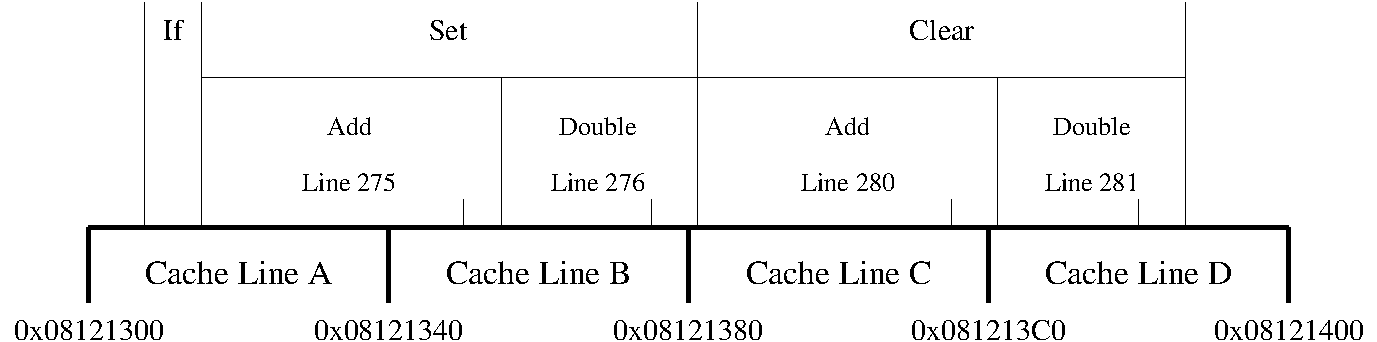
\includegraphics[width=\columnwidth]{images/memory}
\caption{Mapping from Source Code to Memory\label{dgm:memory}}
\end{figure}


The minimum sequence of memory line accesses required for executing this code can now be constructed.
The \texttt{if} statement at line~273 is executed for each bit.  
The code of this statement is in memory line $A$, hence this line is accessed when processing of a bit starts.
For set bit, the processing continues with source line~275, which maps to memory lines~$A$ and~$B$.
The actual call to the group add function occurs at address 0x08121347.
(See mark in Fig.~\ref{dgm:memory}.)
After a delay for computing the group add, execution continues in memory line~$B$ to process the return value and 
to invoke the group doubling function.
The group doubling function returns to memory line~$B$ and execution leaves the \texttt{if} body at memory line~$D$.

Hence, the sequence of memory line accesses required for a set bit is: $A$, $B$, \textit{add}, $B$, \textit{double}, $B$, $D$.
Similarly, for a clear bit, the sequence is: $A$, $C$, \textit{add}, $C$, $D$, \textit{double}, $D$.

Due to the limited temporal resolution of \textsc{Flush+Reload}, the attack can observe the order of memory accesses only
if they are sufficiently separated in time.
Hence, in the case of OpenSSL, the attack can only observe the order of memory accesses if they are separated by a call
to a group operation.
For example, when the bit is set, the attack cannot decide whether the access to memory line~$A$ precedes or follows the access
to memory line~$B$.
Similarly, when observed by \textsc{Flush+Reload}, memory accesses issued after the group double are merged with those 
issued at the start of processing the following bit.
Figure~\ref{dgm:temporal} shows the memory accesses observable by \textsc{Flush+Reload} when processing a set bit followed by
a clear bit.

\begin{figure}[htb]
\centering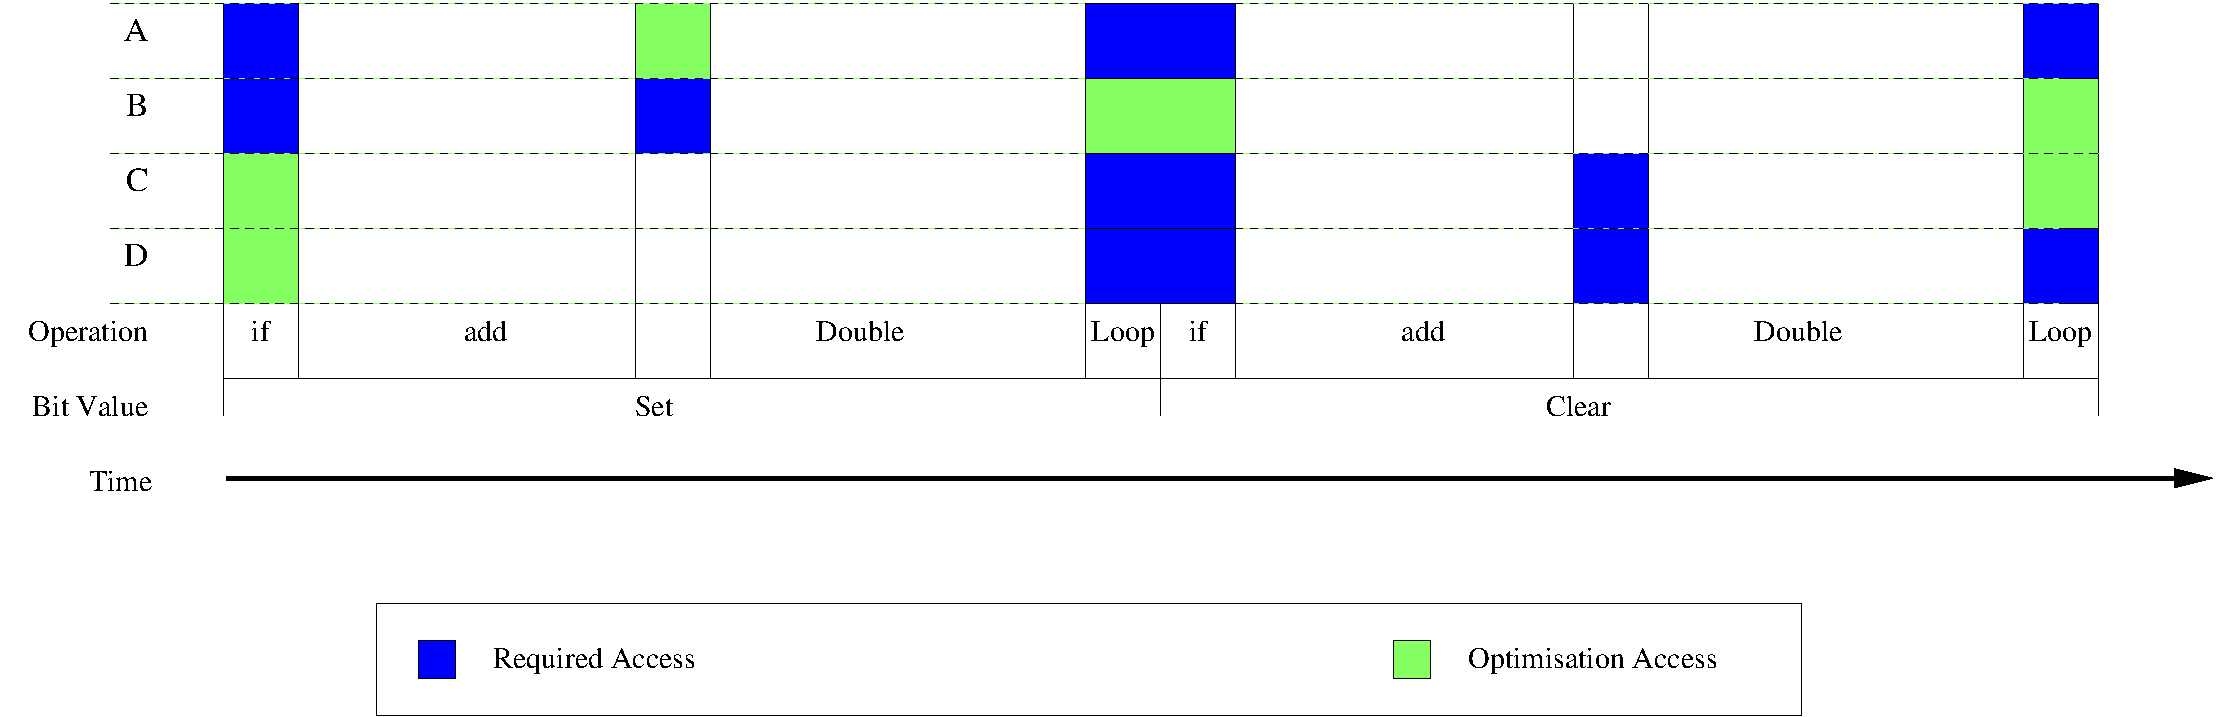
\includegraphics[width=\columnwidth]{images/temporal}
\caption{Observable Memory Access over Time\label{dgm:temporal}}
\end{figure}

The diagram also shows memory accesses issued by processor optimisations.
These optimisations pre-load memory lines into the cache to reduce the time the program waits for these lines.
For example, when the processor uses speculative execution~\cite{uht95disjoint}, it follows both arms of a conditional
branch before evaluating the condition.
When the condition is evaluated, the processor commits to the pre-processed computation of the correct arm,
disposing of the computation done for the other arm. 
In the case of OpenSSL this means that even before evaluating the bit, 
the processor may start processing both line~275 and line~280, triggering memory loads from memory lines~$A$, $B$ and $C$.

Another optimisation that can cause additional memory line access is spatial prefetching~\cite{intel12optimization}.
The processor pairs adjacent memory lines and tries to bring both memory lines into the cache
when there is a miss on one of the pair's line.
For example, when there is a cache miss on memory line~$A$, the spatial prefetcher may attempt to prefetch memory line~$B$
and vice versa.

Consequently, as demonstrated in Fig.~\ref{dgm:temporal}, the memory lines accessed between computing
the group add and the group double can be used for recovering the value of the bit.
Probing any of lines~$A$ and~$B$ gives a positive indication of set bits.  
Probing and of lines~$C$ and~$D$ gives a positive indication of clear bits.
For our attack we probe memory lines~$B$ and~$D$.

Two limitations of the \textsc{Flush+Reload} attack affect its ability to capture the sequence of memory access.
The first is the attack temporal resolution which affect its ability to accurately capture the sequence of memory access
by the victim and the second is the possibility of overlap between the memory access and the probe which may result
in the attack missing the access.

For OpenSSL, the attack resolution should be sufficiently high for the attack to be able to distinguish between 
memory access done before and after each bit and those done between the group add and group double operations of each bit.
This can be achieved by setting the time slot size to be less than the time it takes the victim to calculate the group double.
As group double calculations are faster than group add calculations, this ensures that the probed memory lines are flushed
when the victim computes the group add to be probed when the victim computes the group double.

The probability of overlap, like the attack resolution, depends on the length of the time slot.
Longer time slots mean that the portion of time during which the spy probes is smaller and, therefore, 
the probability of overlap is lower.

Missing memory accesses not only prevents the spy program from recovering the value of bits.
It may also result in the spy program losing the bit position in the scalar multiplication process.
To protect against this possibility, our attack also probes the first and last memory lines of the 
\texttt{gf2m\_Mdouble} function.
Probing these lines provides the spy program with additional information on the operation of the victim
and facilitates recovering the position of captured scalar bits.



The next section describes the details of our experiment with the attack and its results.


\section{Experimental Setup and Results}\label{sec:results}

To test the attack on OpenSSL we used an HP Elite 8300 
running Fedora 18.
As the openssl shipped with Fedora does not support elliptic curves cryptography,
we used our own build of OpenSSL 1.0.1e. 
To facilitate the mapping from source lines to memory addresses we built OpenSSL with debugging symbols.
In a real attack settings, the attacker will need to reverse engineer~\cite{cipsero10software}
the OpenSSL library.
For the experiment we used the OpenSSL \texttt{sect1571r1} curve (NIST Binary-Curve B-571~\cite{fips}.)

With the selected curve, group add operations take 23,612 cycles on average.
The first group double operation takes 6,552 cycles on average, whereas further group double operations take 11,962 cycles.
Consequently, we picked a slot length of 10,240 cycles.

Figure~\ref{dgm:timing} shows the results of the probes during 50 time slots.
Probes taking less than 120 clock cycles indicate a victim access to the probed line.
The diagram also indicates the time slots in which the victim program executed the group add and the group double operations.


\begin{figure}[htb]
\centering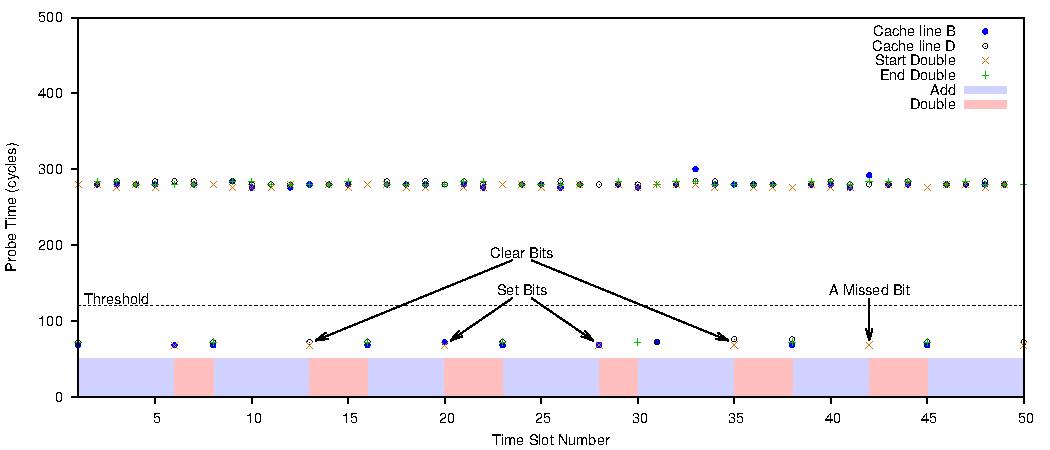
\includegraphics[width=\columnwidth]{images/timing}
\caption{Probe Timing During Signing\label{dgm:timing}}
\end{figure}

For example, in the first time slot, the spy program captured access to memory lines~$B$ and~$D$, as well as an access
to the last memory line of the group double.
The end of the group double is also the end of processing a bit, hence at time slot~1, the victim finished processing a bit
and started the next one.
The next captured probe is at time slot~5.
In this time slot, the victim accessed memory line~$B$ and started executing a group double.  
processing the next bit starts at time slot~8 and ends in time slot~16.
The access to memory line~$D$ in time slot~13 indicates that the second bit is clear.

In the absence access to memory lines~$B$ or~$D$ in time slot~42, the captured access to the group double start indicates
that the spy process missed a value of a bit.
However, the fact that a bit was processed at that time slot is not missed,
demonstrating the value of probing the start of the group double operation.

To measure the number of missing bits we traced the computation of~100 signatures.
on average, the attack misses $4.26\%$ of the bits or $25.28$ bits per signature.
The distribution of number of bits missing per signature is in Fig.~\ref{dgm:dist}(A).
The number of missing bits ranges from 10 to 34, with the median at 25 missing bits per signature.


\begin{figure}[htb]
\begin{tabular}{ccc}
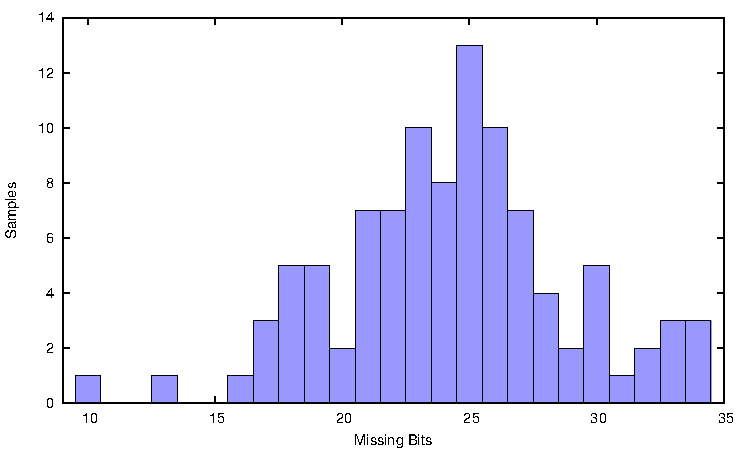
\includegraphics[width=2.4in]{images/missing} &\hfill &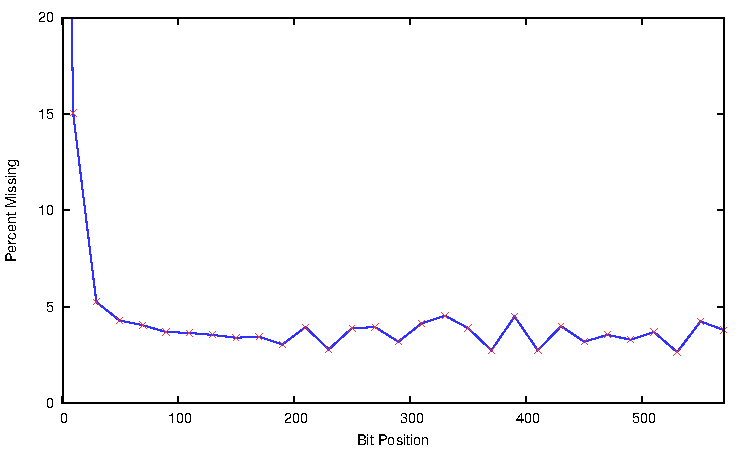
\includegraphics[width=2.4in]{images/positions}\\
(A)& & (B)
\end{tabular}
\caption{Distributions of missing bits: (A) per signature (B) per bit position\label{dgm:dist}}
\end{figure}

As Fig.~\ref{dgm:dist}(B) demonstrates, the distribution of missing bits position is not uniform.
The first bit (bit 0) is always missed.
This is mostly the result of the short time it takes OpenSSL to compute the group double operation for the first bit.
Even ignoring the first bit, it is evident that missing bits tend to cluster towards the most significant bits of the
scalar.
15\% of bits~1 to~20 are missed, compared with 3.6\% of bits from position 50 and up.





\section{Discussion}\label{sec:discussion}
<<<<<<< HEAD
\starpar{LLL attack}
\starpar{Distribution of missing bits} There is a peak initially then the missing bits appear to 
\starpar{Expected number of observed signatures to break key}
=======

\subsection{Full Recovery of the Nonce}\label{sub:full_nonce}
Given the high proportion of nonce bits recovered by the \textsc{Flush+Reload} attack, using the techniques
described in Sect.~\ref{sec:related} seems computationally excessive. 
With a worst case of 34 bits missing, the baby steps giant steps~\cite{shanks71class} would require less then 10 Megabytes of memory
and less than one second of computation to complete the nonce.

There are a number of attacks on ECC protocols which recover the secret key using a small proportion of the leaked nonce. In this attack, the proportion of the nonce recovered by the \textsc{Flush+Reload} attack is significantly higher; using one of the existing attacks would be unnecessarily (computationally) excessive. Attacks using lattice techniques to solve the related hidden number problem, for example, ... 
In experiments a basic BSGS implementation sufficed... 


>>>>>>> 5aff1691280461ac6cd6e8d08fd2c2f6029fbf22


\subsection*{Mitigation}
As the ECDLP is not targeted by this attack, the signature protocol it is made no more vulnerable by our results. This attack is targets the scalar multiplication implementation of OpenSSL and is therefore particular to implementations using 

In the Networking and Cryptography library (NaCl), implemented by Daniel J. Bernstein, Tanja Lange and Peter Schwabe, there is no data flow from secrets to branch conditions, precisely the vulnerability of the OpenSSL implementation targeted by this attack. Analysis of the core security features of NaCl is given in \cite{dan-tan-peter} . The attack presented in this article relies on distinguishing bits of the nonce by observing the branching in traditional Montgomery ladder implementation. As the NaCl library avoids branching dependent on secret parameters this attack is not applicable to NaCl's \url{crypto_sign} API. (NaCl is in the public domain and has been made available by the authors of \cite{dan-tan-peter} at \url{http://nacl.cr.yp.to}.)


\section{Conclusions and future work}
<<<<<<< HEAD
The results of this work and \cite{brumley11remote} imply that the OpenSSL montgomery ladder implementation should be avoided in all implementations of elliptic curve protocols when a scalar multiplication step involves a secret parameter. This attack is applicable when the mallicious party has access to the memory of the targeted device which is not a completely unreasonable assumption ***. 

The results of this work also support the theory of~\cite{walter04longer} that smaller keys are more resilient to side-channel analysis, in this attack a higer proportion of the nonce was obtained for larger key sizes. This implies that as we naturally transition to larger parameters in response to increasing computing capabilities, prevention of side-channel attacks should be incorporated into the implementation design, as is the methodology adopted by the authors of the NaCl cryptographic library. 

There are a number of future directions for this research, including the development of the use of Gray codes in improving the BSGS method to extend the efficiency of obtaining the full scalar from a partially obtained secret. It would also be usedful to understand what proportion of the nonce should be obtained for the BSGS method to become more practical than the LLL method. 

Another related area of interest is how to adapt this attack to recover bits when a sliding window is used; using the method presented in this paper we are able to extract the first and last bit of the sliding window (two bits per window) and thus the proportion of bits obtained decreases as the window size increases. 



=======
The results of this work and \cite{remote_attack} imply that the OpenSSL montgomery ladder implementation should be avoided in all implementations of elliptic curve protocols when a scalar multiplication step involves a secret parameter. This attack is applicable when the malicious party has access to the memory of the targeted device which is not a completely unreasonable assumption ***. 

The results of this work also support the theory of~\cite{walter04longer} that smaller keys are more resilient to side-channel analysis, in this attack a higher proportion of the nonce was obtained for larger key sizes. This implies that as we naturally transition to larger parameters in response to increasing computing capabilities, prevention of side-channel attacks should be incorporated into the implementation design, as adopted by the authors of the NaCl cryptographic library. 
>>>>>>> 5aff1691280461ac6cd6e8d08fd2c2f6029fbf22


\section*{Acknowledgements}
The authors wish to thank Dr Katrina Falkner for the advice and support.

This research was performed under contract to the Defence
Science and Technology Organisation (DSTO) Maritime Division,
Australia.

%\starpar{Bitcoin uses ECDSA}~\cite{nakamoto--bitcoin}

\bibliographystyle{splncs}
\bibliography{Euro2014}

\end{document}

